%%%%%%%%%%%%%%%%%%%%%%%%%%%%%%%%%%%%%%%%%%%%%%%%%%%%%%%%%%%%%%%%%%%%%%%%%%%%%%%%%%%%%%%%%%%%%%%%%%%%%%
%
%   Filename    : appendix_A.tex 
%
%   Description : This file is one of the appendices. 
%                 
%%%%%%%%%%%%%%%%%%%%%%%%%%%%%%%%%%%%%%%%%%%%%%%%%%%%%%%%%%%%%%%%%%%%%%%%%%%%%%%%%%%%%%%%%%%%%%%%%%%%%%

\chapter{Diagrams and Other Documentation Tools}
\label{sec:appendixa}

\section{Process Flow}

\subsection*{The system has two parts: client and server.}


\subsection{Client Side}

The client is implemented on an android tablet. The client is responsible for taking pictures, segmenting it to relevant parts and extracting the relevant information as strings. OpenCV will be used as the primary library for image operations and Tesseract as the primary library for Optical character recognition.


\begin{figure}[h]                %-- use [t] to place figure at top, [b] to place at the bottom, [h] for here
	%-- use this to center the figure
	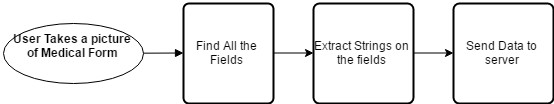
\includegraphics{client.png}      %-- include image file named as "disneychart.png" 
	\caption{Client Side}
	\label{fig:disneystock}
\end{figure}

\pagebreak
\subsection{Server Side} 

The server side is responsible for storing the data received from the client. MySQL will be used as the database and the server side will be implemented on java. 

\begin{figure}[h]                %-- use [t] to place figure at top, [b] to place at the bottom, [h] for here
	\centering                    %-- use this to center the figure
	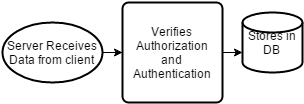
\includegraphics{server.png}      %-- include image file named as "disneychart.png" 
	\caption{Server Side}
	\label{fig:disneystock}
\end{figure}

\pagebreak

\section{Medical Examination Forms currently used by the GetBetter Tele-Diagnosis System.}

\subsection{First Form} 
\begin{figure}[h]                %-- use [t] to place figure at top, [b] to place at the bottom, [h] for here
	\centering                    %-- use this to center the figure
	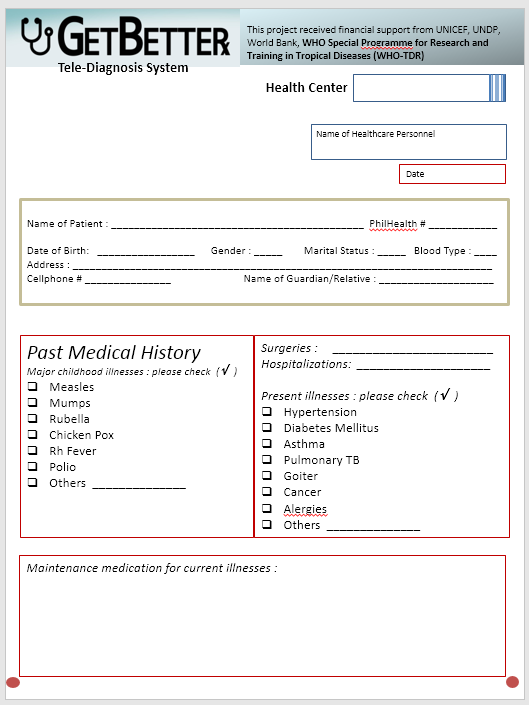
\includegraphics{form1.png}      %-- include image file named as "disneychart.png" 
	\label{}
\end{figure}

\pagebreak
\subsection{Second Form}
\begin{figure}[h]                %-- use [t] to place figure at top, [b] to place at the bottom, [h] for here
	\centering                    %-- use this to center the figure
	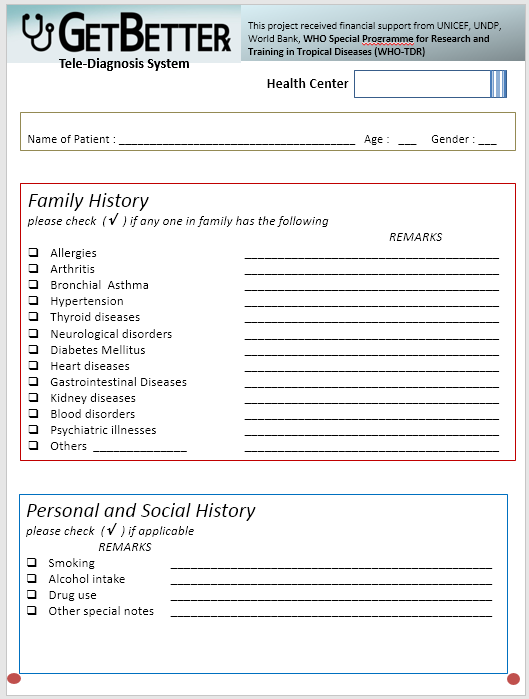
\includegraphics{form2.png}      %-- include image file named as "disneychart.png" 
	\label{}
\end{figure}

\pagebreak
\subsection{Third Form}
\begin{figure}[h]                %-- use [t] to place figure at top, [b] to place at the bottom, [h] for here
	\centering                    %-- use this to center the figure
	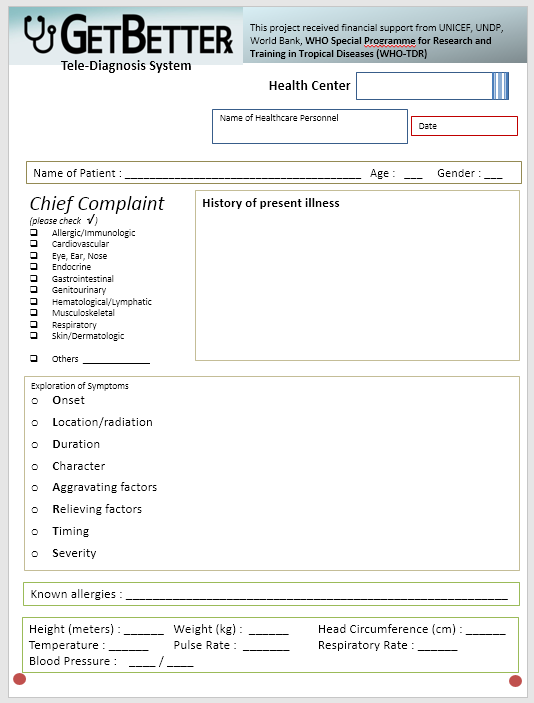
\includegraphics{form3.png}      %-- include image file named as "disneychart.png" 	
	\label{}
\end{figure}


\pagebreak

\section{Medical Examination Forms in preparation for the Optical Character Recognition system}

\subsection{First Form} 
\begin{figure}[h]                %-- use [t] to place figure at top, [b] to place at the bottom, [h] for here
	\centering                    %-- use this to center the figure
	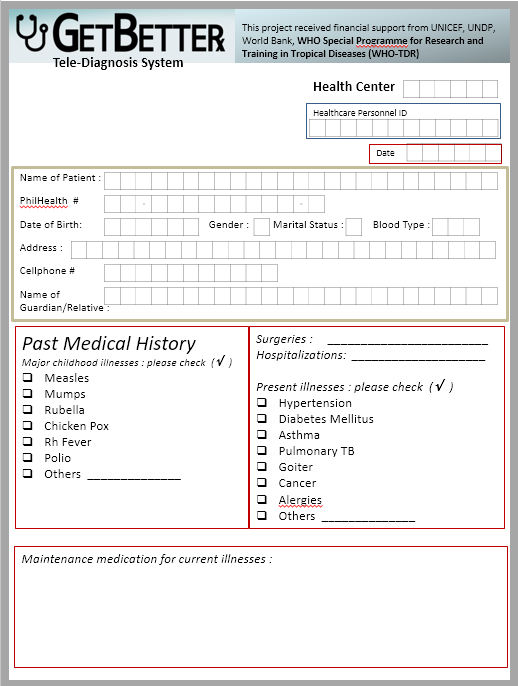
\includegraphics{_newform1.png}      %-- include image file named as "disneychart.png" 
	\label{}
\end{figure}

\pagebreak
\subsection{Second Form}
\begin{figure}[h]                %-- use [t] to place figure at top, [b] to place at the bottom, [h] for here
	\centering                    %-- use this to center the figure
	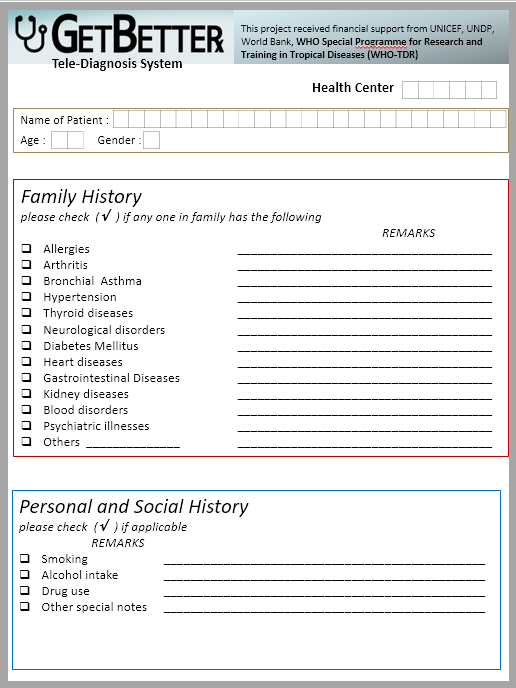
\includegraphics{_newform2.png}      %-- include image file named as "disneychart.png" 
	\label{}
\end{figure}

\pagebreak
\subsection{Third Form}
\begin{figure}[h]                %-- use [t] to place figure at top, [b] to place at the bottom, [h] for here
	\centering                    %-- use this to center the figure
	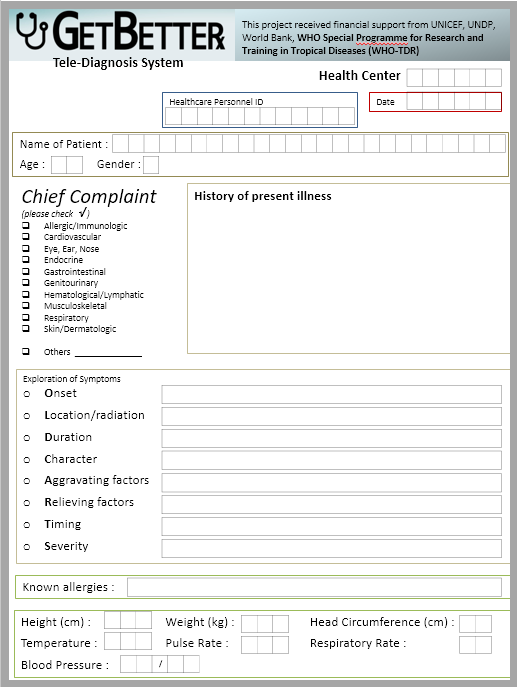
\includegraphics{_newform3.png}      %-- include image file named as "disneychart.png" 	
	\label{}
\end{figure}

\pagebreak
\subsection{Fourth Form}
\begin{figure}[h]                %-- use [t] to place figure at top, [b] to place at the bottom, [h] for here
	\centering                    %-- use this to center the figure
	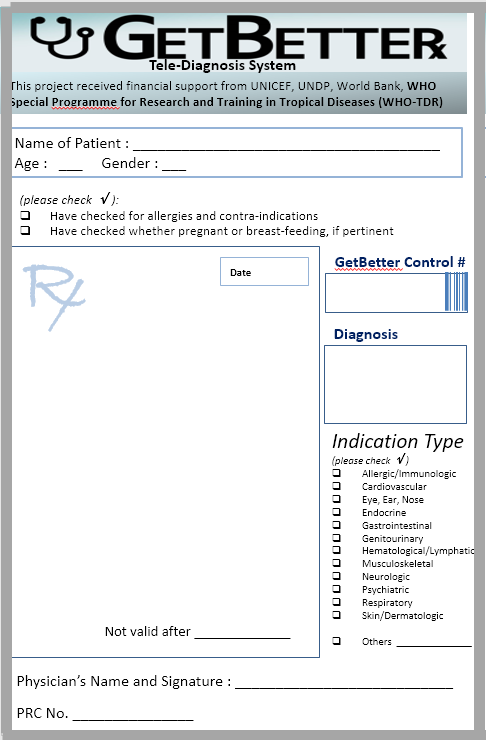
\includegraphics{_newform4.png}      %-- include image file named as "disneychart.png" 	
	\label{}
\end{figure}

\pagebreak
\subsection{Fifth Form}
\begin{figure}[h]                %-- use [t] to place figure at top, [b] to place at the bottom, [h] for here
	\centering                    %-- use this to center the figure
	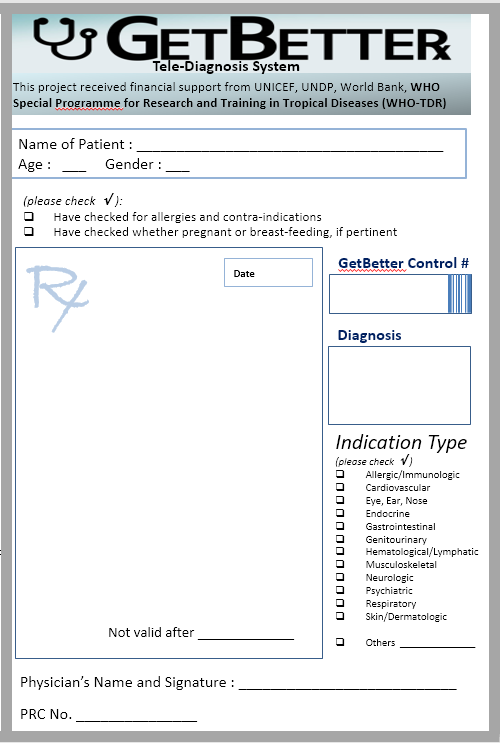
\includegraphics{_newform5.png}      %-- include image file named as "disneychart.png" 	
	\label{}
\end{figure}








